\documentclass{article}\usepackage[]{graphicx}\usepackage[]{color}
%% maxwidth is the original width if it is less than linewidth
%% otherwise use linewidth (to make sure the graphics do not exceed the margin)
\makeatletter
\def\maxwidth{ %
  \ifdim\Gin@nat@width>\linewidth
    \linewidth
  \else
    \Gin@nat@width
  \fi
}
\makeatother

\definecolor{fgcolor}{rgb}{0.345, 0.345, 0.345}
\newcommand{\hlnum}[1]{\textcolor[rgb]{0.686,0.059,0.569}{#1}}%
\newcommand{\hlstr}[1]{\textcolor[rgb]{0.192,0.494,0.8}{#1}}%
\newcommand{\hlcom}[1]{\textcolor[rgb]{0.678,0.584,0.686}{\textit{#1}}}%
\newcommand{\hlopt}[1]{\textcolor[rgb]{0,0,0}{#1}}%
\newcommand{\hlstd}[1]{\textcolor[rgb]{0.345,0.345,0.345}{#1}}%
\newcommand{\hlkwa}[1]{\textcolor[rgb]{0.161,0.373,0.58}{\textbf{#1}}}%
\newcommand{\hlkwb}[1]{\textcolor[rgb]{0.69,0.353,0.396}{#1}}%
\newcommand{\hlkwc}[1]{\textcolor[rgb]{0.333,0.667,0.333}{#1}}%
\newcommand{\hlkwd}[1]{\textcolor[rgb]{0.737,0.353,0.396}{\textbf{#1}}}%

\usepackage{framed}
\makeatletter
\newenvironment{kframe}{%
 \def\at@end@of@kframe{}%
 \ifinner\ifhmode%
  \def\at@end@of@kframe{\end{minipage}}%
  \begin{minipage}{\columnwidth}%
 \fi\fi%
 \def\FrameCommand##1{\hskip\@totalleftmargin \hskip-\fboxsep
 \colorbox{shadecolor}{##1}\hskip-\fboxsep
     % There is no \\@totalrightmargin, so:
     \hskip-\linewidth \hskip-\@totalleftmargin \hskip\columnwidth}%
 \MakeFramed {\advance\hsize-\width
   \@totalleftmargin\z@ \linewidth\hsize
   \@setminipage}}%
 {\par\unskip\endMakeFramed%
 \at@end@of@kframe}
\makeatother

\definecolor{shadecolor}{rgb}{.97, .97, .97}
\definecolor{messagecolor}{rgb}{0, 0, 0}
\definecolor{warningcolor}{rgb}{1, 0, 1}
\definecolor{errorcolor}{rgb}{1, 0, 0}
\newenvironment{knitrout}{}{} % an empty environment to be redefined in TeX

\usepackage{alltt}
\setlength\parindent{0pt}
\usepackage{geometry}

%This is word 'normal' margins
\geometry{left=1.25in,right=1in,top=1.25in,bottom=1.25in}
\IfFileExists{upquote.sty}{\usepackage{upquote}}{}
\begin{document}



\section*{Problem 1}
\subsection*{i}
We will use BIC to select the best model.
\begin{knitrout}
\definecolor{shadecolor}{rgb}{0.969, 0.969, 0.969}\color{fgcolor}\begin{kframe}
\begin{alltt}
\hlcom{# best subset}
\hlstd{s} \hlkwb{=} \hlstd{leaps::}\hlkwd{regsubsets}\hlstd{(medv} \hlopt{~} \hlstd{.,} \hlkwc{data} \hlstd{= Boston,} \hlkwc{method} \hlstd{=} \hlstr{"exhaustive"}\hlstd{,} \hlkwc{nvmax} \hlstd{=} \hlkwd{ncol}\hlstd{(Boston)} \hlopt{-}
    \hlnum{1}\hlstd{)}
\hlstd{s}  \hlcom{#forward}
\hlstd{f} \hlkwb{=} \hlstd{Rcmdr::}\hlkwd{stepwise}\hlstd{(}\hlkwd{lm}\hlstd{(medv} \hlopt{~} \hlstd{.,} \hlkwc{data} \hlstd{= Boston),} \hlkwc{direction} \hlstd{=} \hlstr{"forward"}\hlstd{,} \hlkwc{criterion} \hlstd{=} \hlstr{"BIC"}\hlstd{)}
\hlcom{# backward}
\hlstd{b} \hlkwb{=} \hlstd{Rcmdr::}\hlkwd{stepwise}\hlstd{(}\hlkwd{lm}\hlstd{(medv} \hlopt{~} \hlstd{.,} \hlkwc{data} \hlstd{= Boston),} \hlkwc{direction} \hlstd{=} \hlstr{"backward"}\hlstd{,} \hlkwc{criterion} \hlstd{=} \hlstr{"BIC"}\hlstd{)}
\hlcom{# best model for backward selection and best subset selection}
\hlstd{sb} \hlkwb{=} \hlkwd{glm}\hlstd{(medv} \hlopt{~} \hlstd{crim} \hlopt{+} \hlstd{zn} \hlopt{+} \hlstd{chas} \hlopt{+} \hlstd{nox} \hlopt{+} \hlstd{rm} \hlopt{+} \hlstd{dis} \hlopt{+} \hlstd{rad} \hlopt{+} \hlstd{tax} \hlopt{+} \hlstd{ptratio} \hlopt{+} \hlstd{black} \hlopt{+}
    \hlstd{lstat,} \hlkwc{data} \hlstd{= Boston)}
\hlcom{# best moel for forward selection}
\hlstd{f} \hlkwb{=} \hlkwd{glm}\hlstd{(medv} \hlopt{~} \hlstd{lstat} \hlopt{+} \hlstd{rm} \hlopt{+} \hlstd{ptratio} \hlopt{+} \hlstd{dis} \hlopt{+} \hlstd{nox} \hlopt{+} \hlstd{chas} \hlopt{+} \hlstd{black} \hlopt{+} \hlstd{zn,} \hlkwc{data} \hlstd{= Boston)}
\end{alltt}
\end{kframe}
\end{knitrout}


We can see the selected models in the above code. Best subset selection and backward selection choose medv~crim + zn + chas + nox + rm + dis + rad + tax + ptratio + black + lstat while forward selection chooses medv ~ lstat + rm + ptratio + dis + nox + chas + black + zn.

\subsection*{ii}
\begin{knitrout}
\definecolor{shadecolor}{rgb}{0.969, 0.969, 0.969}\color{fgcolor}\begin{kframe}
\begin{alltt}
\hlcom{# 5 fold cv MSE for best subset/backwards regression model}
\hlkwd{set.seed}\hlstd{(}\hlnum{12345}\hlstd{)}
\hlstd{boot::}\hlkwd{cv.glm}\hlstd{(Boston, sb,} \hlkwc{K} \hlstd{=} \hlnum{5}\hlstd{)}\hlopt{$}\hlstd{delta[}\hlnum{1}\hlstd{]}
\end{alltt}
\begin{verbatim}
## [1] 23.58
\end{verbatim}
\begin{alltt}
\hlcom{# 5 fold cv MSE for forwards selection model}
\hlkwd{set.seed}\hlstd{(}\hlnum{12345}\hlstd{)}
\hlstd{boot::}\hlkwd{cv.glm}\hlstd{(Boston, f,} \hlkwc{K} \hlstd{=} \hlnum{5}\hlstd{)}\hlopt{$}\hlstd{delta[}\hlnum{1}\hlstd{]}
\end{alltt}
\begin{verbatim}
## [1] 24.38
\end{verbatim}
\end{kframe}
\end{knitrout}


Using this seed the best subset/backwards selection model medv~crim + zn + chas + nox + rm + dis + rad + tax + ptratio + black + lstat performs better.

\clearpage

\section*{Problem 3}
\subsection*{i}
\begin{knitrout}
\definecolor{shadecolor}{rgb}{0.969, 0.969, 0.969}\color{fgcolor}\begin{kframe}
\begin{alltt}
\hlstd{enzyme} \hlkwb{=} \hlkwd{read.table}\hlstd{(}\hlstr{"Enzyme.txt"}\hlstd{,} \hlkwc{head} \hlstd{= T)}
\hlstd{enzyme.prime} \hlkwb{=} \hlnum{1}\hlopt{/}\hlstd{enzyme}
\hlstd{alpha} \hlkwb{=} \hlkwd{coef}\hlstd{(}\hlkwd{lm}\hlstd{(Y} \hlopt{~} \hlstd{x,} \hlkwc{data} \hlstd{= enzyme.prime))}
\hlstd{beta} \hlkwb{=} \hlkwd{as.numeric}\hlstd{(}\hlkwd{c}\hlstd{(}\hlnum{1}\hlopt{/}\hlstd{alpha[}\hlnum{1}\hlstd{], alpha[}\hlnum{2}\hlstd{]}\hlopt{/}\hlstd{alpha[}\hlnum{1}\hlstd{]))}
\hlstd{beta}
\end{alltt}
\begin{verbatim}
## [1] 29.62 13.45
\end{verbatim}
\end{kframe}
\end{knitrout}


The initival values of $\beta$ are 29.622, 13.4488
\subsection*{ii}
\begin{knitrout}
\definecolor{shadecolor}{rgb}{0.969, 0.969, 0.969}\color{fgcolor}\begin{kframe}
\begin{alltt}
\hlstd{m0} \hlkwb{=} \hlkwd{nls}\hlstd{(}\hlkwc{formula} \hlstd{= Y} \hlopt{~} \hlstd{b0} \hlopt{*} \hlstd{x}\hlopt{/}\hlstd{(b1} \hlopt{+} \hlstd{x),} \hlkwc{data} \hlstd{= enzyme,} \hlkwc{start} \hlstd{=} \hlkwd{c}\hlstd{(}\hlkwc{b0} \hlstd{= beta[}\hlnum{1}\hlstd{],}
    \hlkwc{b1} \hlstd{= beta[}\hlnum{2}\hlstd{]))}
\hlkwd{coef}\hlstd{(m0)}
\end{alltt}
\begin{verbatim}
##    b0    b1 
## 28.14 12.57
\end{verbatim}
\end{kframe}
\end{knitrout}

The OLS estimtates of $\beta$ are 28.137, 12.5745
\subsection*{iii}
\begin{knitrout}
\definecolor{shadecolor}{rgb}{0.969, 0.969, 0.969}\color{fgcolor}\begin{kframe}
\begin{alltt}
\hlkwd{plot}\hlstd{(enzyme}\hlopt{$}\hlstd{x, enzyme}\hlopt{$}\hlstd{Y)}
\hlkwd{lines}\hlstd{(enzyme}\hlopt{$}\hlstd{x,} \hlkwd{fitted.values}\hlstd{(m0))}
\end{alltt}
\end{kframe}

{\centering 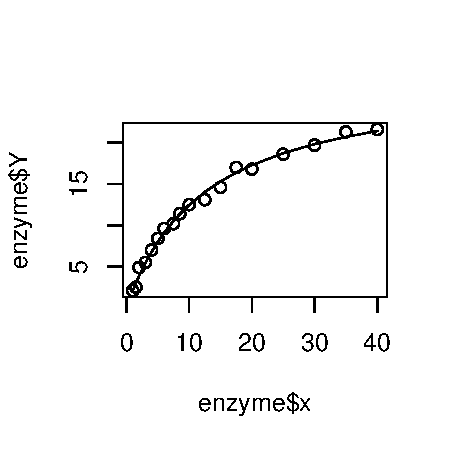
\includegraphics[width=\maxwidth]{figure/unnamed-chunk-6} 

}



\end{knitrout}

The fit is adequate.

\subsection*{iv}
\begin{knitrout}
\definecolor{shadecolor}{rgb}{0.969, 0.969, 0.969}\color{fgcolor}\begin{kframe}
\begin{alltt}
\hlkwd{plot}\hlstd{(enzyme}\hlopt{$}\hlstd{x,} \hlkwd{resid}\hlstd{(m0))}
\hlkwd{plot}\hlstd{(}\hlkwd{fitted.values}\hlstd{(m0),} \hlkwd{resid}\hlstd{(m0))}
\end{alltt}
\end{kframe}
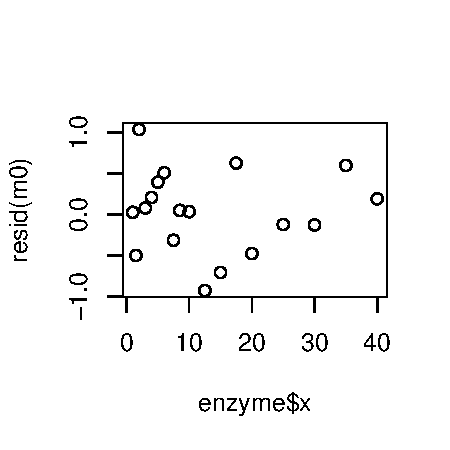
\includegraphics[width=\maxwidth]{figure/unnamed-chunk-71} 
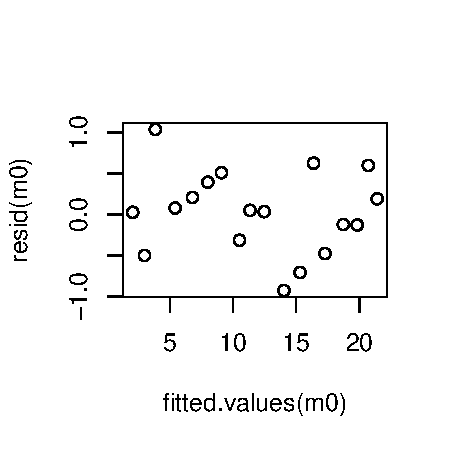
\includegraphics[width=\maxwidth]{figure/unnamed-chunk-72} 

\end{knitrout}


\begin{knitrout}
\definecolor{shadecolor}{rgb}{0.969, 0.969, 0.969}\color{fgcolor}\begin{kframe}
\begin{alltt}
\hlkwd{qqnorm}\hlstd{(}\hlkwd{resid}\hlstd{(m0))}
\hlkwd{qqline}\hlstd{(}\hlkwd{resid}\hlstd{(m0))}
\end{alltt}
\end{kframe}

{\centering 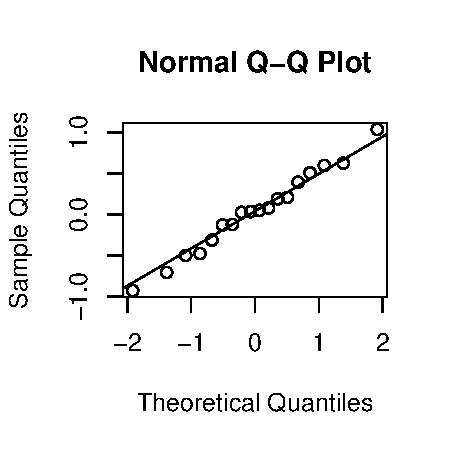
\includegraphics[width=\maxwidth]{figure/unnamed-chunk-8} 

}



\end{knitrout}


These plots seem to show that our model is a good fit. The first two plots show no obvious patterns and small residuals. The QQ plot seems to show that our residuals are normally distributed.
\subsection*{v}
Although there is no hypothesis test with null 'this is a bad model' or 'this is not a bad model', there are many ways to test if the resdiauls are normally distributed which is a more formal way to check if that particular assumption holds than a qq plot. According to (NM Razali, YB Wah, 2012) the Shapiro–Wilk test is the highest power test of normality.

\begin{knitrout}
\definecolor{shadecolor}{rgb}{0.969, 0.969, 0.969}\color{fgcolor}\begin{kframe}
\begin{alltt}
\hlkwd{shapiro.test}\hlstd{(}\hlkwd{resid}\hlstd{(m0))}\hlopt{$}\hlstd{p}
\end{alltt}
\begin{verbatim}
## [1] 0.9943
\end{verbatim}
\end{kframe}
\end{knitrout}


We see that the p-value is 0.9943 and thus fail to reject that the residuals are normally distributed.
\subsection*{vi}
If we collect more datapoints that are closer together (or indeed replications) then we will have lower standard error and thus lower confidence and prediction intervals locally around the points we have sampled. If we collect data points that are farther apart (and no replications) then we will not have as small of a local standard error, confidence intervals, or prediction intervals, but at each concentration value, but we know more about a larger range of concentration values. There will always be a tradeoff between local precision and trying to get a more global view of the phenomenon. 
\subsection*{vii}
\subsubsection*{1}
\begin{knitrout}
\definecolor{shadecolor}{rgb}{0.969, 0.969, 0.969}\color{fgcolor}\begin{kframe}
\begin{alltt}
\hlstd{est} \hlkwb{=} \hlkwd{summary}\hlstd{(m0)}\hlopt{$}\hlstd{coefficients[}\hlnum{1}\hlstd{,} \hlnum{1}\hlstd{]}
\hlstd{sd} \hlkwb{=} \hlkwd{summary}\hlstd{(m0)}\hlopt{$}\hlstd{coefficients[}\hlnum{1}\hlstd{,} \hlnum{2}\hlstd{]}
\hlstd{ci} \hlkwb{=} \hlkwd{c}\hlstd{(est} \hlopt{-} \hlnum{1.96} \hlopt{*} \hlstd{sd, est} \hlopt{+} \hlnum{1.96} \hlopt{*} \hlstd{sd)}
\hlstd{ci}
\end{alltt}
\begin{verbatim}
## [1] 26.71 29.56
\end{verbatim}
\end{kframe}
\end{knitrout}

The 95\% confidence interval is 26.7102, 29.5639.

\subsubsection*{2}
\begin{knitrout}
\definecolor{shadecolor}{rgb}{0.969, 0.969, 0.969}\color{fgcolor}\begin{kframe}
\begin{alltt}
\hlstd{est} \hlkwb{=} \hlkwd{summary}\hlstd{(m0)}\hlopt{$}\hlstd{coefficients[}\hlnum{1}\hlstd{,} \hlnum{1}\hlstd{]}
\hlstd{sd} \hlkwb{=} \hlkwd{summary}\hlstd{(m0)}\hlopt{$}\hlstd{coefficients[}\hlnum{1}\hlstd{,} \hlnum{2}\hlstd{]}
\hlstd{pval} \hlkwb{=} \hlnum{1} \hlopt{-} \hlkwd{pchisq}\hlstd{(((est} \hlopt{-} \hlnum{20}\hlstd{)}\hlopt{/}\hlstd{sd)}\hlopt{^}\hlnum{2}\hlstd{,} \hlnum{1}\hlstd{)}
\hlstd{pval}
\end{alltt}
\begin{verbatim}
## [1] 0
\end{verbatim}
\end{kframe}
\end{knitrout}

The p-value is 0

\section*{Problem 4} 
\subsection*{a}
Based on the analysists reasons we can not conclude that the model is highly effective for producing prediction ingervals for suggested retail price. We can only say that dealer cost as significantly correlated with suggested retail price. There are many reasons that this is in fact a bad model which I will discuss in the following sections.
\subsection*{b}
In the plot of the studentized residuals vs the predictor we see that there is a heteroskedacity problem and our residuals vairance increases as the dealer cost increases. We also can see a clear increasing trend in the square root of the residuals vs the dealer cost. showing that we will make larger errors as the price of the cars increase. The qqplot is also very poor  in the two extremes showing that there are many outliers that are vasly underpriced or overpriced in the model.
\subsection*{c}
The new model seems to perform better than the old one. The studentized residuals show less outliers and the plot vs the predictor shows less of a pattern. The square root of the residuals vs the predictor now shows no trend. There are still a few outliers and these can be seen in the normal QQ plot, indicating that this model may still not be as good as we may like.
\subsection*{d}
If the dealer cost increases by 1\% then the suggested retail price will increase by $\beta_1$\%
\subsection*{e}
We still see that there are a few studentized residuals with large negative values when the dealer cost is low. This means that our model may underprice some low cost cars. The interpretation of the model is also much less clear than the first model. If this model will not be used by a computer to set the price in advance, but rather is going to be used to give the sales people quick and simple insights into reasonable prices of the cars then it may not be very good.

\section*{Problem 5}

\subsection*{a}
This model contains two insignificant variables (hybrid and wheelbase) which should be removed (remove one at a time, maybe removing one will make the other significant) and is thus not a 'valid' model. We should always aim for more parsimonious modes if possible. We also see from the diagnoistic plots that the model does not fit very well. In particular we see that there are a few very large residuals for high priced cars indicating that we are going to underprice expensive cars.
\subsection*{b}
From the curve in the plot we see that we will tend to underprice very cheap and very expensive cars. Cars with average prices will tend to be priced better.
\subsection*{c}
According to wikipedia there are three main heuristics to use Cook's distance to classify if points have high influence or not, $D_i>1$, $D_i>4/n$ and $D_i>F_{p,n-p,1-\alpha}$. We have $4/n=$0.0171 and $F_{p,n-p,1-\alpha} =$ 1.9795. Using a cutoff of 1, or $D_i>F_{p,n-p,1-\alpha}$ we find no highly influential points. Using a cutoff of $4/n$ we find theat most points are highly influental. We will conclude that there are no highly influential points.
\subsection*{d}
This model contains two non significant predictors (thighwaympg and twheelbase) which should be removed (remove one at a time, maybe removing one will make the other significant) and is thus not a 'valid' model. We should always aim for more parsimonious modes if possible. THe diagnoistic plots are better than before but still not quite satisfying.

\subsection*{e}

\subsection*{f}
Add j-1 new predictors where j is the number of unique manufacturers, each variable will be an indicator if the car is one of j-1 specific manufacturer, and if all the variables are 0 then the car will be the reaming manufacturer. We may wish to do further analysis to see if we can collapse several brands into one category (for example luxury car vs non luxury car).

\end{document}
